%%%%%%%%%%%%%%%%%%%%%%%%%%%%%%%%%%%%%%%%%
% Jacobs Landscape Poster
% LaTeX Template
% Version 1.1 (14/06/14)
%
% Created by:
% Computational Physics and Biophysics Group, Jacobs University
% https://teamwork.jacobs-university.de:8443/confluence/display/CoPandBiG/LaTeX+Poster
% 
% Further modified by:
% Nathaniel Johnston (nathaniel@njohnston.ca)
%
% This template has been downloaded from:
% http://www.LaTeXTemplates.com
%
% License:
% CC BY-NC-SA 3.0 (http://creativecommons.org/licenses/by-nc-sa/3.0/)
%
%%%%%%%%%%%%%%%%%%%%%%%%%%%%%%%%%%%%%%%%%

%----------------------------------------------------------------------------------------
%	PACKAGES AND OTHER DOCUMENT CONFIGURATIONS
%----------------------------------------------------------------------------------------

\documentclass[final]{beamer}

\usepackage[scale=1.24]{beamerposter} % Use the beamerposter package for laying out the poster

\usetheme{confposter} % Use the confposter theme supplied with this template

\setbeamercolor{block title}{fg=ngreen,bg=white} % Colors of the block titles
\setbeamercolor{block body}{fg=black,bg=white} % Colors of the body of blocks
\setbeamercolor{block alerted title}{fg=white,bg=dblue!70} % Colors of the highlighted block titles
\setbeamercolor{block alerted body}{fg=black,bg=dblue!10} % Colors of the body of highlighted blocks
% Many more colors are available for use in beamerthemeconfposter.sty

%-----------------------------------------------------------
% Define the column widths and overall poster size
% To set effective sepwid, onecolwid and twocolwid values, first choose how many columns you want and how much separation you want between columns
% In this template, the separation width chosen is 0.024 of the paper width and a 4-column layout
% onecolwid should therefore be (1-(# of columns+1)*sepwid)/# of columns e.g. (1-(4+1)*0.024)/4 = 0.22
% Set twocolwid to be (2*onecolwid)+sepwid = 0.464
% Set threecolwid to be (3*onecolwid)+2*sepwid = 0.708

\newlength{\sepwid}
\newlength{\onecolwid}
\newlength{\twocolwid}
\newlength{\threecolwid}
\setlength{\paperwidth}{48in} % A0 width: 46.8in
\setlength{\paperheight}{36in} % A0 height: 33.1in
\setlength{\sepwid}{0.024\paperwidth} % Separation width (white space) between columns
\setlength{\onecolwid}{0.22\paperwidth} % Width of one column
\setlength{\twocolwid}{0.464\paperwidth} % Width of two columns
\setlength{\threecolwid}{0.708\paperwidth} % Width of three columns
\setlength{\topmargin}{-0.00000005in} % Reduce the top margin size
%-----------------------------------------------------------

\usepackage{graphicx}  % Required for including images

\usepackage{booktabs} % Top and bottom rules for tables
\renewcommand{\arraystretch}{1.2} 

%----------------------------------------------------------------------------------------
%	TITLE SECTION 
%----------------------------------------------------------------------------------------

\title{Duluth at SemEval-2017 Task 6: Language Models in Humor Detection} % Poster title

\author{\textbf{Xinru Yan \& Ted Pedersen} \\ 
\vspace{4mm}
\normalsize \href{mailto:\{yanxx418,tpederse\}@d.umn.edu}{\{yanxx418,tpederse\}@d.umn.edu} \\
\vspace{4mm} 
\normalsize \href{https://xinru1414.github.io/HumorDetection-SemEval2017-Task6/}{https://xinru1414.github.io/HumorDetection-SemEval2017-Task6/}} % Author(s)

\institute{Department of Computer Science University of Minnesota Duluth} % Institution(s)


%----------------------------------------------------------------------------------------

\begin{document}

\addtobeamertemplate{block end}{}{\vspace*{2ex}} % White space under blocks
\addtobeamertemplate{block alerted end}{}{\vspace*{2ex}} % White space under highlighted (alert) blocks

\setlength{\belowcaptionskip}{1ex} % White space under figures
\setlength\belowdisplayshortskip{3ex} % White space under equations

\begin{frame}[t] % The whole poster is enclosed in one beamer frame

\begin{columns}[t] % The whole poster consists of three major columns, the second of which is split into two columns twice - the [t] option aligns each column's content to the top

\begin{column}{\sepwid}\end{column} % Empty spacer column

\begin{column}{\onecolwid} % The first column

%----------------------------------------------------------------------------------------
%	INTRODUCTION
%----------------------------------------------------------------------------------------

\begin{block}{Introduction}

SemEval-2017 Task 6 \textit{\#HashtagWars: Learning a Sense of Humor} aims to characterize humor from tweets submitted to a game show \textit{@midnight} \cite{PotashRR17}.
Duluth system completed the task using \textbf{Ngram Language Models (LMs)} \cite{Heafield-estimate}.

%------------------------------------------------

\begin{figure}

\includegraphics[width=0.9\linewidth]{@midnight.jpg}
% \caption{Figure caption}
\end{figure}


%----------------------------------------------------------------------------------------

\end{block}

%----------------------------------------------------------------------------------------
%	Background
%----------------------------------------------------------------------------------------

\begin{block}{Language Models}
\begin{itemize}
%\item \textbf{Ngram}: a contiguous sequence of N words
\item \textbf{Ngram models}: predict the upcoming word from the previous N-1 words.
\item \textbf{Markov} assumption: the probability (PR) of a word depends only on a small number of previous words. For trigrams:
\begin{equation}
P(w_n|w_1^{n-1})\approx P(w_n|w_{n-2}, w_{n-1})
\end{equation}
\item \textbf{Trigram LM}: use trigrams to compute the PR of a sequence of words:
\begin{equation}
P(w_1^n)\approx \prod_{k=1}^{n} P(w_k|w_{k-2}, w_{k-1})
\end{equation}
\item We train LMs to assess the \textbf{similarity} of a tweet comparing to funny tweets, or \textbf{distinctiveness} of a tweet comparing to the \textbf{common language} (English news) to detect how humorous it is \cite{hello}.
\end{itemize}
\end{block}

\begin{center}
\begin{tabular}{c}

\includegraphics[width=0.7\linewidth]{logo.png}\\
\end{tabular}
\end{center}

\end{column} % End of the first column

\begin{column}{\sepwid}\end{column} % Empty spacer column

\begin{column}{\twocolwid} % Begin a column which is two columns wide (column 2)

%----------------------------------------------------------------------------------------
%	Task
%----------------------------------------------------------------------------------------

\begin{block}{The Task}
Tweets are in three baskets: top most funny tweet, next nine funny tweets and all remaining.%tweets. There are two subtasks involved:
\begin{itemize}
\item Subtask A: Pairwise Comparison -- a system should predict which tweet is funnier for every possible combination of tweet pairs from a given hashtag file.
\item Subtask B: Semi-Ranking -- a system should produce a ranking of tweets from funniest to the least funny for a specific hashtag file. 
\end{itemize}
\end{block}



%----------------------------------------------------------------------------------------
%	IMPORTANT RESULT
%----------------------------------------------------------------------------------------

\begin{alertblock}{Examples from \#BreakUpIn5Words (Trigram LM, News Data)}

\begin{table}[h!]
\centering
\begin{tabular} {  p{30cm} | p{10cm} | p{10cm} }
\toprule
\multicolumn{1}{c|}{\Large Tweet} & \Large \textit{@midnight} & \Large Duluth \\
\hline
\Large It's not you, it's meth. & \Large funniest & \Large funny \\
\Large Hey, can we NOT talk? & \Large funny & \Large funny \\
\Large You need your own Netflix  & \Large funny & \Large not funny \\
\Large Figured I'd try being happy.  & \Large not funny & \Large funny \\
\Large You're a Mac, I'm PC & \Large not funny & \Large not funny \\	
\bottomrule
\end{tabular}
\end{table}
\end{alertblock}


\begin{columns}[t,totalwidth=\twocolwid] % Split up the two columns wide column

\begin{column}{\onecolwid}\vspace{-.6in} % The first column within column 2 (column 2.1)

%----------------------------------------------------------------------------------------- 
% 	Method
%-----------------------------------------------------------------------------------------

\begin{block}{Method}

%------------------------------------------------

\begin{figure}
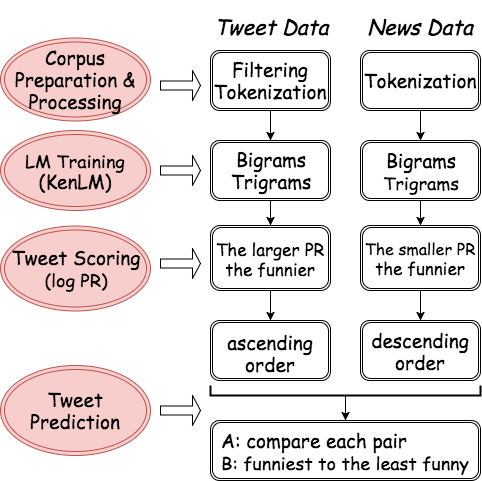
\includegraphics[width=1.04\linewidth]{Method.png} 
% \caption{Figure caption}
\end{figure}


%---------------------------------------------------------------------------------------

\end{block}


\end{column}


\begin{column}{\onecolwid}\vspace{-.6in} % The second column within column 2 (column 2.2)



%----------------------------------------------------------------------------------------
%	Dataset
%----------------------------------------------------------------------------------------

\begin{block}{Dataset}
\begin{itemize}
\item \textbf{Tweet Data}: provided by the task, 106 hashtag files, about 21,580 tokens.
\item \textbf{News Data}: We used 6.2 GB English news, about 2 million tokens \cite{EMNLP}.
\end{itemize}
\end{block}

\begin{block}{Results}

\begin{table}[h!]
\centering
\begin{tabular}{ |p{5cm}|p{4.5cm}|p{8.5cm}|p{8cm}|}
\toprule
\multicolumn{1}{|c|}{Dataset} & \multicolumn{1}{|c|} {Ngram} & Accuracy (A) & Distance (B) \\
\hline
\multicolumn{1}{|c|}{\textbf{news}} & \multicolumn{1}{|c|}{\textbf{3}} & \textbf{0.627} (4th) & \textbf{0.872} (1st)\\
\hline
\multicolumn{1}{|c|}{news} & \multicolumn{1}{|c|}{2} & 0.624 & 0.853 \\
\hline
\multicolumn{1}{|c|}{\textbf{tweet}} & \multicolumn{1}{|c|}{\textbf{3}} & \textbf{0.397} (8th) & \textbf{0.967} (8th)\\
\hline
\multicolumn{1}{|c|}{tweet} & \multicolumn{1}{|c|}{2} & 0.406 & 0.944 \\
\bottomrule
\end{tabular}
\end{table}
\end{block}

\end{column}

\end{columns}


\end{column} % end of the second column

\begin{column}{\sepwid}\end{column} % Empty spacer column

\begin{column}{\onecolwid} % The third column

%----------------------------------------------------------------------------------------
%	Discussion
%----------------------------------------------------------------------------------------

\begin{block}{Discussion \& Future Work}
\begin{itemize}
\item Duluth relied on bigram and trigram LMs since tweets are \textbf{short} and \textbf{concise}
\item Bigram LMs performed slightly better than trigram LMs: 
\\ --> \textit{Unigram} and \textit{character} level LMs 
\item The \textbf{type} and the \textbf{quantity} of the corpora is what really matters: 
\\ --> \textit{more tweet data, less news data}
\item Duluth did extremely well on
\vspace{3mm} 
\\\#BreakUpIn5Words by using trigram LM trained on news data and performed
\vspace{3mm}
\\the worst on \#RuinAChristmasMovie: 
%One possible reason could be that
\begin{itemize} 
\item \large Language in \#BreakUpIn5Words is the least similar to news compared to other hashtags thus represented better;  
\item \large LMs do not have external knowledge such as movie titles.
\end{itemize}
\item Traditional Ngram models do not 
\vspace{3mm}
\\account for long distance dependencies
\vspace{3mm} 
\\and creative use of language (OOV).
\vspace{3mm}
\\-->\textit{Deep learning method}: 
\begin{itemize}
\large \item LSTMs: long term dependencies
\large \item Character-based CNNs: unknown words
\end{itemize}
\end{itemize}
\end{block}


%----------------------------------------------------------------------------------------
%	REFERENCES
%----------------------------------------------------------------------------------------

\begin{block}{References}

\nocite{*} % Insert publications even if they are not cited in the poster
\tiny{\bibliographystyle{unsrt}
\bibliography{sample}\vspace{0.75in}}

\end{block}
%\tiny \footnotetext[1]{http://www.statmt.org/wmt11/translation-task.html}



%----------------------------------------------------------------------------------------

\end{column} % End of the third column


\end{columns} % End of all the columns in the poster



\end{frame} % End of the enclosing frame

\end{document}
